\documentclass[a4paper, 12pt]{article}
\usepackage[brazil]{babel}  	  % nomes de seções e títulos em Pt-BR
\usepackage[utf8]{inputenc} 	  % codificação de texto compatível com Pt-BR
\usepackage[T1]{fontenc}
\usepackage{physics, mathtools}
\usepackage{amsmath, amssymb, amsthm, amsfonts} % pacotes da AMS para ambientes matemáticos
\usepackage[final]{microtype} %melhora a tipografia do texto.
\usepackage{hyperref} % cria hyperlinks para equações, teoremas, etc
%\usepackage{showlabels} Mostra os nomes dos labels.
\usepackage{graphicx, color}      % pacote para a inclusao de figuras em jpg, pdf, png e textos coloridos
\usepackage{epstopdf, epsfig}	  % pacote para a conversao de eps para pdf
\usepackage{latexsym}
\usepackage{subfigure, wrapfig}
\usepackage{indentfirst}
\usepackage[table]{xcolor}
\usepackage{tabularx, scalefnt}
\usepackage{multicol, multirow}
\usepackage{calc}
\usepackage{ifthen}
\usepackage{pdfpages}
\usepackage{fancyhdr}
\usepackage{circuitikz}
\usepackage{url}
\usepackage{lastpage}
\usepackage[top=3cm, left=3cm, right=2cm, bottom=2cm]{geometry}

\begin{document}

% CRIANDO A CAPA DO RELATÓRIO DE FÍSICA EXPERIMENTAL

\begin{center}
	
\includegraphics[scale=0.08]{./pictures/brasao.png}\\
{\footnotesize {\bf MINISTÉRIO DA EDUCAÇÃO\\
	SECRETARIA DE EDUCAÇÃO PROFISSIONAL, CIENTÍFICA E TECNOLÓGICA\\
	INSTITUTO FEDERAL DE EDUCAÇÃO, CIÊNCIA E TECNOLOGIA CATARINENSE\\
	\textit{CAMPUS} SÃO BENTO DO SUL\\
	BACHARELADO EM ENGENHARIA DE COMPUTAÇÃO}}

\vspace{5cm}
\textbf{TÍTULO DO RELATÓRIO DO EXPERIMENTO}

\vspace{3cm}
\begin{tabular}{|l|l|}
\hline
{\bf Disciplina:} Física Experimental II & {\bf Turma:} ECA2024/2 \\ \hline
{\bf Professor:} Genilson Carvalho & genilson.carvalho@ifc.edu.br \\ \hline
{\bf Responsável:} Nelson Dias Ponciano Scarin & nelsonscarin34@gmail.com \\ \hline
Nome e Sobrenome & e-mail \\ \hline
Nome e Sobrenome & e-mail \\ \hline
Nome e Sobrenome & e-mail \\ \hline
Nome e Sobrenome & e-mail \\ \hline
\end{tabular}

\vspace{7cm}
São Bento do Sul - SC\\
\today
\end{center}
\newpage	

% INICIANDO O RELATÓRIO	
\twocolumn[
\begin{center}
	\textbf{TÍTULO DO RELATÓRIO DO EXPERIMENTO}
\end{center}
\vspace{0.5cm}
\begin{center}
\begin{minipage}{16.0cm}
	\textbf{RESUMO.} {\it Este é o resumo do relatório. O resumo deve ser objetivo, coerente e curto, com aproximadamente 100 palavras. Com a leitura deste resumo qualquer pessoa tem que ser capaz de entender o trabalho desenvolvido pelo grupo e a que resultados chegaram. Estas instruções tem como objetivo guiá-lo na preparação de seu relatório no formato de artigo científico.}\\
	\textbf{Palavras-chave:} Relatório; Resultados; Artigo científico.
\end{minipage}
\end{center}]

\section{Introdução}\label{intro}
A introdução deve situar o leitor no assunto. Em geral, em artigos científicos, a introdução contém um histórico do que já foi desenvolvido sobre o assunto, os resultados relevantes existentes na literatura, e em função disto esta é a seção que contem o maior número de citações. Outro componente da introdução, que é o que nos interessa, é o embasamento teórico sobre o assunto estudado, isto é, onde se explica a física ou a química envolvida. Em ambos os casos isto não significa uma mera listagem de fórmulas e equações envolvidas no experimento. Na introdução deve também existir um parágrafo que relaciona o experimento feito ao contexto teórico~\cite{Fisica-II}.

Os autores devem preparar seus relatórios seguindo este padrão apresentado, que já vem pré-formatado. Isto deverá facilitar muito e certamente vai auxiliá-los no domínio desta ferramenta de edição de texto.
Estes relatórios deverão ser enviados por e-mail em formato PDF, dentro do prazo pré-estabelecido. Relatórios entregues fora do prazo ou assinados por alunos que não realizaram a atividade experimental perderão pontos~\cite{Halliday-II}.

O relatório deverá possuir, no mínimo, duas e, no máximo, cinco folhas, sendo que deverá ser feito com letra preta em folhas brancas (os gráficos podem ser em cores). Caso for impresso, deverá ser feito, se possível em frente e verso, em papel de tamanho A4, empregando o formato aqui mostrado.

\begin{table}
\centering
\caption{Este é um exemplo de formatação de tabela~\cite{michael}.}
\scalefont{0.9}
\begin{tabular}{|c|c|c|}
\hline
Kelvin (K) & Celsius (ºC) & Fahrenheit (ºF) \\ \hline
271 & 2 & 31 \\ \hline
274 & 5 & 36 \\ \hline
277 & 8 & 39 \\ \hline
281 & 11 & 42 \\ \hline
\end{tabular}\\
\label{table1}
\end{table}

Lembre-se de colocar a figura e a tabela~\ref{table1} centralizadas na coluna assim como seus textos descritivos (legendas). Esses textos descritivos devem ser sucintos, objetivos e claros de forma que a pessoa que vê a figura ou tabela saiba do que se trata.

\section{Metodologia}
Nesta seção são descritos os procedimentos empregados para efetuar as medidas e são descritas as montagens experimentais utilizadas. Diagramas esquemáticos das experiências são bastante úteis pois facilitam a visualização.  Este procedimento NÃO é uma cópia do roteiro do experimento pois o mesmo não contém detalhes relevantes que somente podem ser percebidos durante a elaboração da experiência. Lembre-se que seu leitor deve ser capaz de reproduzir o experimento a partir da leitura desta seção e da seção~\ref{intro}.

\section{Resultados e Discussões}
Esta seção é o coração do relatório. Nela são apresentados os dados obtidos em forma de tabelas, gráficos e diagramas. Lembre-se que quando o volume de dados é elevado os gráficos devem ter preferência sobre as tabelas. Os resultados experimentais devem ser confrontados com as previsões teóricas e com os resultados existentes na literatura citada na introdução. Quando são efetuados cálculos complexos não é necessário descrever todas as etapas do processo. No caso dos resultados experimentais, dentro das estimativas de erro, apresentarem discrepâncias com as previsões teóricas o procedimento experimental deverá ser reavaliado (isto porque no nosso caso os resultados são muito bem conhecidos). Na vida real pode ocorrer discrepância devido às falhas dos modelos teóricos existentes, ou das medidas feitas previamente. Lembre-se que toda medida experimental apresenta incerteza e portanto as contas efetuadas devem levar estas em consideração.

\begin{figure}[!htpb]
	\centering
	\caption{Velocidade em função do tempo.}
	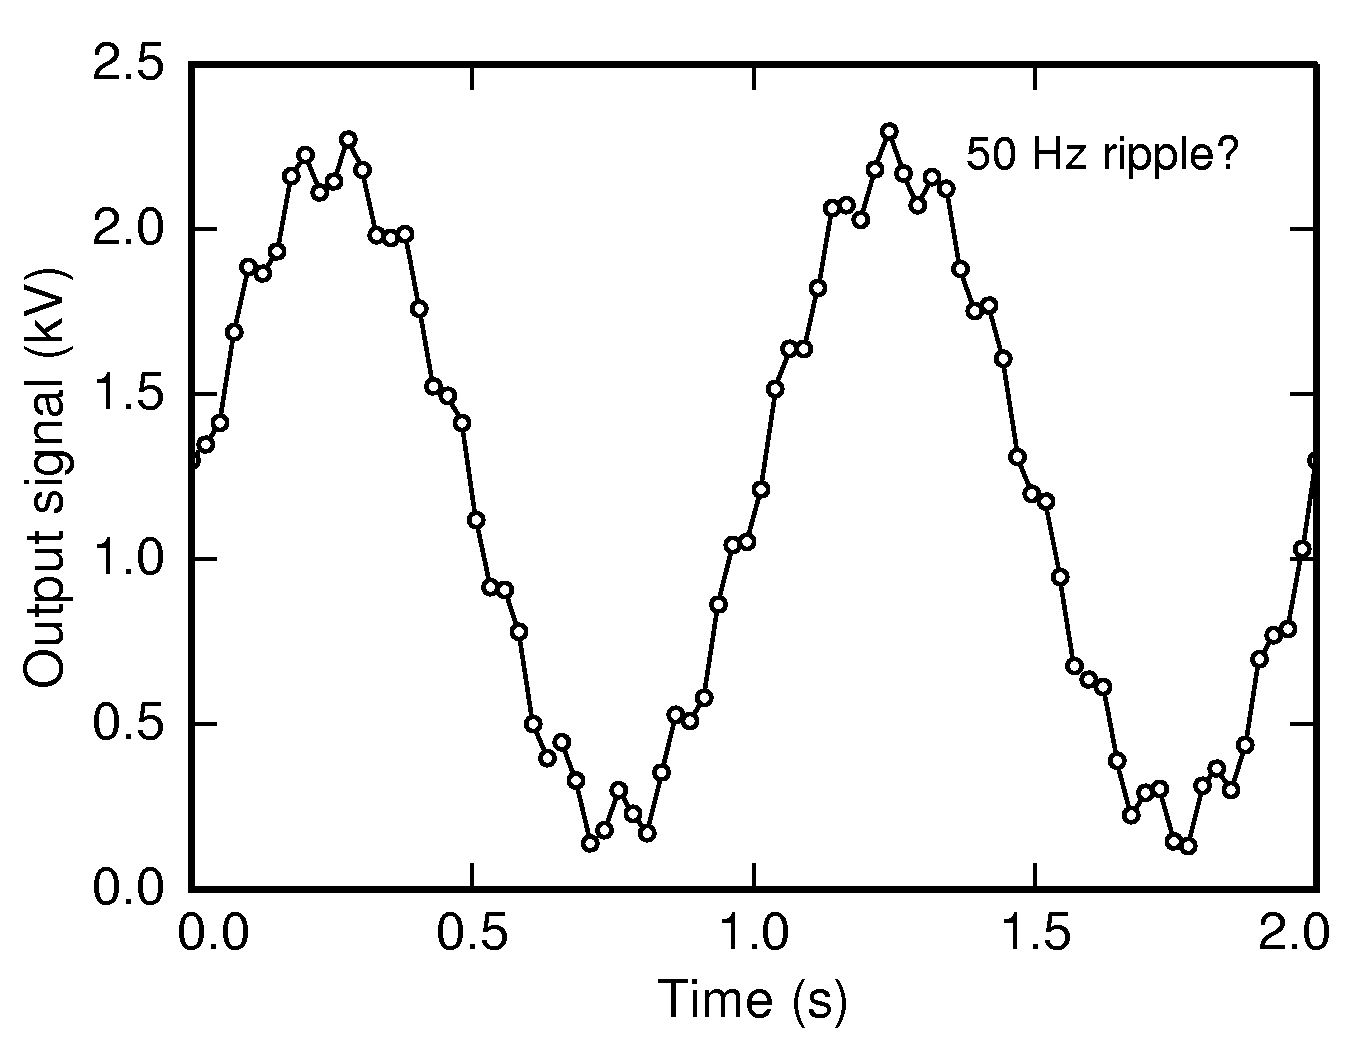
\includegraphics[scale=0.15]{./pictures/grafico1.png}
	Fonte: Adaptado do Halliday e Resnick~\cite{Halliday-II}.
\end{figure}

\section{Conclusão}
A conclusão deve abordar brevemente o experimento efetuado, os resultados obtidos e a que conclusões estes resultados levam. Em alguns casos se discute possíveis rumos desta investigação. Comentários do tipo: ``O experimento foi muito proveitoso$\dots$'' e outro similares deve ser evitados.

%\onecolumn

\bibliographystyle{unsrt}
\bibliography{biblio.bib}

\end{document}